%INITIAL
%class
	\PassOptionsToPackage{dvipsnames}{xcolor}
	\documentclass[hideothersubsections]{beamer}

%template
	\usetheme{_SalmanHannover}
	%\usecolortheme{rose}
	\setbeamertemplate{navigation symbols}{\insertbackfindforwardnavigationsymbol, \insertframenavigationsymbol}
%\insertslidenavigationsymbol%
%\insertframenavigationsymbol%
%\insertsubsectionnavigationsymbol%
%\insertsectionnavigationsymbol%
%\insertdocnavigationsymbol%
%\insertbackfindforwardnavigationsymbol

	%\setbeamertemplate{footline}	{\tiny{\vspace{0in}\hspace{4.3in}\Acrobatmenu{GoBack}{\beamerreturnbutton{back}}\hspace{0.05in}\color{blue}\insertframenumber/\inserttotalframenumber}} 

	%\setbeamertemplate{footline}{\centering{\insertframenumber/\insertpresentationendpage}}
	%\setbeamertemplate{footline}{\hspace*{.5cm}\scriptsize{\hfill\insertframenumber\hspace*{.5cm}}} 


%packages
	\usepackage{amsmath, amssymb, mathrsfs, graphicx,cancel,bigints,wrapfig}
%\usepackage{media9}
%\usepackage{animate}
	\usepackage[absolute,overlay]{textpos}
	\usepackage{tikz}
	\usetikzlibrary{calc, shapes}
	\usepackage{totcount}
	\usepackage{subfigure,soul}
	\usepackage{pgfpages}
%\usepackage{titlesec}\titleformat{\section}{\color{red}\normalfont\Large\bfseries}{\color{red}\thesection}{1em}{}
	\usepackage{caption}\captionsetup{labelformat=empty,labelsep=none}
%\setbeamertemplate{caption}[numbered]
%	\usepackage{caption} 
%	\setbeamertemplate{caption}[numbered]
	\usepackage{geometry}
	\geometry{verbose}
	%\usepackage{pifont}
	\usepackage{color}
\definecolor{lightgray}{gray}{0.95}
\usepackage{listings}
\lstset{breaklines=true,
breakindent=0pt,
prebreak=\mbox{\tiny$\searrow$},
postbreak=\mbox{{\color{blue}\tiny$\rightarrow$}},
numbers=left,
commentstyle=\color{darkgreen},
numberblanklines=false,
frame=single,
captionpos=b,
backgroundcolor=\color{lightgray}}
	\usepackage{xmpmulti}
	%\usepackage[3D]{movie15}
	\usepackage{hyperref}
%	\usepackage{bookmark}
	\usepackage[open,openlevel=4,atend]{bookmark}
	%\bookmarksetup{color=blue}
	\usepackage{multirow}
	\usepackage[backend=bibtex, style=numeric,defernumbers, authoryear]{biblatex}
	%\usepackage[square,sort]{natbib}
	%\usepackage{fancyhdr}\pagestyle{fancyplain} 
%\rfoot{\thepage}
	\usepackage{tikz}
	\hypersetup{bookmarksdepth = 4}




%citations files
	\bibliography{MyCitations}

%logoCAE
    \setlength{\TPHorizModule}{1mm}
    \setlength{\TPVertModule}{1mm}
    \newcommand{\logoCAE}
    {
    	\begin{textblock}{1}(115,2.5) %(100,85)  for bottom, (115,1)  for top right
    		
\includegraphics[width=1.2cm]{figs/logo_CAE}
    	\end{textblock}
  
    }

%logoCAE_gray
    \setlength{\TPHorizModule}{1mm}
    \setlength{\TPVertModule}{1mm}
    \newcommand{\logoCAEgray}
    {
    	\begin{textblock}{1}(115,1) %(100,85)  for bottom
    		\includegraphics[width=1.2cm]{figs/logo_CAE_gray.png}
    	\end{textblock}
  
    }


%logo Tech Tower
    \newcommand{\logoTechTower}
    {
    	\begin{textblock}{1}(0,0) 
    		\includegraphics[width=1.25in]{thesis/logo_TechTower.png}
    	\end{textblock}
    }

%logoCSIPCPL
    \setlength{\TPHorizModule}{1mm}
    \setlength{\TPVertModule}{1mm}
    \newcommand{\logoCSIPCPL}
    {
    	\begin{textblock}{1}(100,2) %(100,85)  for bottom
    		
\includegraphics[width=1.5cm]{thesis/logo_CSIP}
    	\end{textblock}
    	
	\begin{textblock}{1}(117,1) %(117,85)  for bottom
    		
\includegraphics[width=1.0cm]{thesis/logo_CPL}
    	\end{textblock} 
    }


%logo tree
    \newcommand{\logoTree}
    {
    	\begin{textblock}{1}(0,0) 
    		\includegraphics[width=1.25in]{figs/logo_tree.jpg}
    	\end{textblock}
    }

%logo tree
    \newcommand{\logoCAEE}
    {
    	\begin{textblock}{1}(0,13) 
    		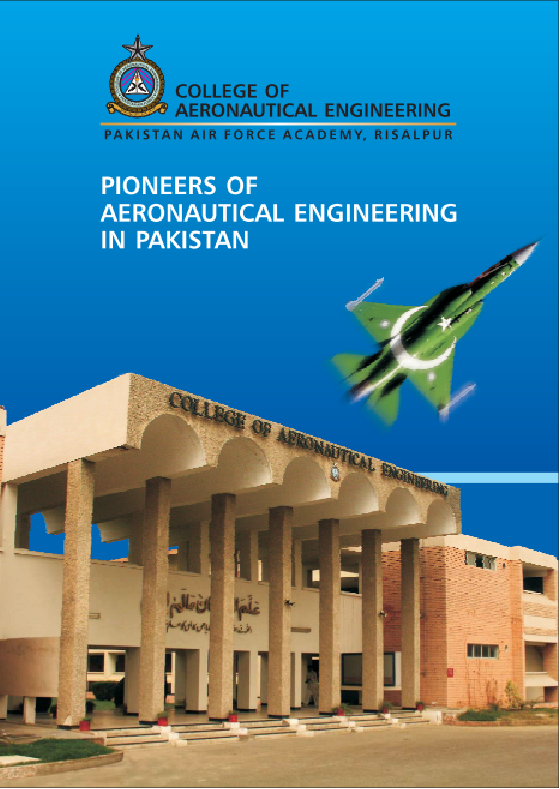
\includegraphics[width=1.7in]{figs/logo_CAE_front.png}
    	\end{textblock}
    }


%logo researchers
    \newcommand{\logoResearchers}
    {
    	\begin{textblock}{1}(0,0) 
    		\includegraphics[width=1.25in]{figs/lecture_SigProc_portrait_researchers.png}
    	\end{textblock}
    }

%page numbers
    \newcommand{\mypagenum}
    {
    	\begin{textblock}{1}(117,0.5)  %bottom right is (110,94)
		{\tiny \color[rgb]{0.2,0.2,1}{\insertframenumber~/~\inserttotalframenumber}} %\insertpresentationendpage, 
    	\end{textblock}
    }




%my footnote citation
	\newcommand{\myFootnoteCitation}[2]
	{
		\footnote{\tiny \citeauthor{#1}, \emph{#2}, \citeyear{#1}.}  %\citeauthor{#1}, \citetitle{#1}, #2 \citeyear{#1}.
	}
%my refer to citation
	\newcommand{\mycite}[1]
	{
		\emph{\citeauthor{#1} (\citeyear{#1})}
	}
%my footnote website citation
	\newcommand{\myFootnoteWebsiteCitation}[1]
	{
		\footnote{\tiny \citeauthor{#1}}
	}

\let\thefootnote\relax\footnotetext{Footnotetext without footnote mark}


%section underline
%\newcommand{\tmpsection}[1]{}
%\let\tmpsection=\section
%\renewcommand{\section}[1]{\tmpsection{\underline{#1}}}


\newenvironment<>{varblock}[2][\textwidth]{
    \begin{center}
      \begin{minipage}{#1}
        \setlength{\textwidth}{#1}
          \begin{actionenv}#3
            \def\insertblocktitle{#2}
            \par
            \usebeamertemplate{block begin}}
  {\par
      \usebeamertemplate{block end}
    \end{actionenv}
  \end{minipage}
\end{center}}


%commands
	\newcommand{\likelihood}{p(Z_k| x_k) }						%likelihood
	\newcommand{\prior}{p(x_k)  } 								%prior
	\newcommand{\posterior} {p(x_k| Z_k)}						%posterior
	\newcommand{\prediction} {p(x_k| Z_{k-1})}					%prediction
	\newcommand{\update} {p(x_k|Z_k)}							%update
	\newcommand{\observations} {p(Z_k)}						%observations
	\newcommand{\prevobservations} {p(Z_{k-1})}				%previous observations
	\newcommand{\dxpk} {dx_{k-1}}							%dx_{k-1}
	\newcommand{\ChapKolm}{\int{p(x_k| x_{k-1})p(x_{k-1}|Z_{k-1})} \dxpk} %Chapman Kolmogorov

	%algorithm specific: JPDAF
	\newcommand{\likelihoodJPDAF}{p(Z_k| \chi, m, Z_{k-1}) }		%1. likelihood
	\newcommand{\priorJPDAF}{p(\chi|m, Z^{k-1}} 				%2. prior	
	\newcommand{\observationsJPDAF} {p(Z_k}					%3. observations
	\newcommand{\posteriorJPDAF} {p(\chi| Z_k)}					%4. posterior

%environments
	\newenvironment{changemargin}[2]
	{
	  	\begin{list}{}
		{
			\setlength{\topsep}{0pt}%
			\setlength{\leftmargin}{#1}%
			\setlength{\rightmargin}{#2}%
			\setlength{\listparindent}{\parindent}%
			\setlength{\itemindent}{\parindent}%
			\setlength{\parsep}{\parskip}%
		}
	  	\item[]
		}
		{\end{list}
	}
%font sizes
\makeatletter
  \newcommand\tinyv{\@setfontsize\tinyv{5pt}{4}}
\makeatother

\makeatletter
  \newcommand\tinyvv{\@setfontsize\tinyvv{8pt}{4}}
\makeatother

\makeatletter
  \newcommand\tinyvs{\@setfontsize\tinyvs{7pt}{4}}
\makeatother


\makeatletter
  \newcommand\tinyvvv{\@setfontsize\tinyvvv{0.5pt}{0.5}}
\makeatother


%booleans
\newboolean{PrintHandout}
\newboolean{ShowOverlays}

%tikz styles
\tikzstyle{mybox} = [draw=red, fill=blue!20, very thick,rectangle, rounded corners, inner sep=10pt, inner ysep=20pt]
\tikzstyle{fancytitle} =[fill=blue, text=white, ellipse]
\tikzstyle{myboxtwo} = [fill=blue!20,rectangle, rounded corners, inner sep=10pt, inner ysep=20pt]

%colors
\definecolor{darkgreen}{rgb}{0,0.5,0}
\definecolor{darkcyan}{rgb}{0,0.5,0.5}
\definecolor{darkbrown}{rgb}{0.65,0.48,0.14}
\definecolor{lightblue}{rgb}{0.58,0.7,0.9}
\definecolor{lightred}{rgb}{0.92,0.52,0.52}

%personal details
	\author{Dr Salman Aslam}
	%\author{Dr Salman Aslam}
	\institute{Wing Commander, PAF\\Associate Professor\\Avionics Department\\College of Aeronautical Engineering\\PAF Academy Risalpur}
	\date{}

\begin{document}
\include{lecture_SigProc_formulas}
\title{WFAR3 (LUMS)}


%CONDITIONAL
\setboolean{PrintHandout}{false}
\mypagenum\ifthenelse{\boolean{PrintHandout}}
{
	\pgfpagesuselayout{4 on 1}[a4paper,border shrink=2mm,landscape] 
}
{
	\setboolean{ShowOverlays}{true}
}

%counters
\newcounter{cnt_Number}\regtotcounter{cnt_Number}
\newcounter{cnt_LogicGates}\regtotcounter{cnt_LogicGates}
\newcounter{cnt_Boolean}\regtotcounter{cnt_Boolean}

%START
\begin{frame}[plain]
\logoCAEE\logoCAE
%\title{3rd German-Pakistani Workshop on Field and Assistive Robotics}
\title{CAE\\Robotics at CAE\\Residual Vector Quantization}
\titlepage
\end{frame}



\begin{frame}
\frametitle{Outline}
\logoCAE
\setcounter{tocdepth}{2}	
\tableofcontents
\end{frame}




%####################################################################################################
\section{Introduction}
%####################################################################################################
%=======================
\subsection{\ \ \ \ Bio}
%=======================

\begin{frame}
\frametitle{Introduction}
\framesubtitle{Bio (salman at gatech.edu)}
\mypagenum\ifthenelse{\boolean{ShowOverlays}}{\logoCAE}{}
\begin{changemargin}{-0.24in}{0in}
\vspace{0.1in}\hspace{0.15in}{\color{red}Education}
\begin{enumerate}\scriptsize
\item 1995: BE, US Air Force Academy (EE)
\item 2008: MS, Georgia Tech (ECE)
\item 2011: PhD, Georgia Tech \emph{\tiny (Target Tracking Using Residual Vector Quantization)}
\item 2012: Associate Professor, CAE
\end{enumerate}


\vspace{0.2in}\hspace{0.15in}{\color{red}Research interests}
\begin{enumerate}\scriptsize
\item PRML: pattern recognition, machine learning
\item signal processing, computer vision
\item robotics
\end{enumerate}

\vspace{0.2in}\hspace{0.15in}{\color{red}Experience}
\begin{enumerate}\scriptsize
\item 1995: US DoD %\emph{\tiny (Washington DC)}
\item 1999: PAF, developed prototype V/UHF Jammer
%\begin{itemize}\scriptsize
%\item PC-bus plug-in hardware
%\item accompanying software
%\item off-the-shelf receivers, tuners, amplifiers
%\item demonstrated in Air Headquarters
%\end{itemize}
\item 2001: PAF, simulation of V/UHF jamming scenario \emph{\tiny (demonstrated in AHQ)}
\item 2002: PAF, Aircraft deployment patterns of IAF fighters \emph{\tiny (CAS appreciation)}
\item 2003: PAF, Radar triangulation system \emph{\tiny (CAS commendation)}
\item 2007: Siemens Global CoC for Intelligent Video %\emph{\tiny (Atlanta)}
\item 2008: Nvidia Video Algorithms Group %\emph{\tiny (Santa Clara)}
\item 2009: Nvidia Video Research Group  %\emph{\tiny (Santa Clara)}
\item 2010: Qualcomm Multimedia Research %\emph{\tiny (San Diego)}
\item 2011: Samsung Research Labs %\emph{\tiny (Dallas)}
\end{enumerate}
\end{changemargin}
\end{frame}








%####################################################################################################
\section{CAE}
%####################################################################################################
%=======================
\subsection{\ \ \ \ History}
%=======================
\begin{frame}
\frametitle{CAE}
\framesubtitle{History}
\mypagenum\ifthenelse{\boolean{ShowOverlays}}{\logoCAE}{}
\begin{figure}
\centering
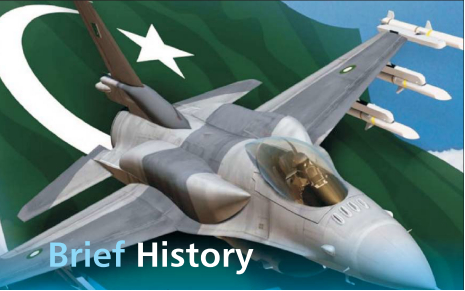
\includegraphics[height=0.3\textheight]{figs/logo_CAE_history.png}
\end{figure}
\begin{itemize}
\item 1965: setup in Korangi Creek, Karachi
\item 1983: moved to PAF Academy, Risalpur
\item 1996: affiliated with NUST
\item 2010: re-accredited by PCE, highest score in country 
\end{itemize}
%\Acrobatmenu{GoBack}{\beamerreturnbutton{back}}
\end{frame}


%=======================
\subsection{\ \ \ \ Departments}
%=======================
\begin{frame}
\frametitle{CAE}
\framesubtitle{Departments}
\mypagenum\ifthenelse{\boolean{ShowOverlays}}{\logoCAE}{}
\begin{enumerate}
\item Avionics Engineering (undergrad degree)
\item Aerospace Engineering (undergrad degree)
\item Industrial Engineering
\item Humanities and Sciences
\item Professional Continuing Education
\end{enumerate}
\end{frame}


%=======================
\subsection{\ \ \ \ Labs}
%=======================
\begin{frame}
\frametitle{CAE}
\framesubtitle{Labs}
\mypagenum\ifthenelse{\boolean{ShowOverlays}}{\logoCAE}{}
\vspace{0.1in}
\scriptsize Avionics
\begin{enumerate}\scriptsize
\item Basic
\item Digital and Embedded Systems
\item Guidance, Navigation, Controls
\item Antenna and Electromagnetic
\item Communications
\item Radar
\item Microwave
\item PCB Prototyping
\item Thermal Imaging
\item Robotics and Computer Vision (set up last month)
\end{enumerate}
\scriptsize Aerospace
\begin{enumerate}\scriptsize
\item Aerodynamics
\item Propulsion and Heat Transfer
\item Structures
\item Materials Science
\item Numerical Analysis
\item Aerospace Project
\end{enumerate}
\scriptsize Industrial Engineering workshop, Physics Lab, Chemistry Lab
\end{frame}








%=======================
\subsection{\ \ \ \ Projects}
%=======================
\begin{frame}
\frametitle{CAE}
\framesubtitle{Avionics Projects}
\mypagenum\ifthenelse{\boolean{ShowOverlays}}{\logoCAE}{}
RF/Microwave
\begin{enumerate}\scriptsize
\item Design and fabrication of a miniaturized phased array antenna for wi-fi application
\item Reverse engineering of RF power amplifier used in radar transmitter module phase-II
\item Design and development of wireless clock synchronization system
\item Design and fabrication of rf front end receiver for software defined radio: (RF part 1)
\item Design and development of a microstrip phased array antenna for electronic beam steering
\item Design and simulation of optical circulator using various numerical algorithms
\end{enumerate}
Laser/IR
\begin{enumerate}\scriptsize
\item Design and experimental demonstration of laser based remote listening technique
\item Design and development of improved IR parameter security system
\end{enumerate}
\end{frame}



\begin{frame}
\frametitle{CAE}
\framesubtitle{Avionics Projects \tiny cont.}
\mypagenum\ifthenelse{\boolean{ShowOverlays}}{\logoCAE}{}
Communications
\begin{enumerate}\scriptsize
\item Development of an IP based voice communication system using open source software PBX on an embedded platform
\item Simulation and evaluation of modulation and channel coding schemes in jamming
\item Design and development of software/digital part ofsoftware defined radio kit: phase II
\item Design and development of an FPGA based cryptographic system
\end{enumerate}
Radars
\begin{enumerate}\scriptsize
\item Design and replacement of digital portion of MPDR-45E radar receiver with an embedded processing platform
\end{enumerate}
\end{frame}



\begin{frame}
\frametitle{CAE}
\framesubtitle{Avionics Projects \tiny cont.}
\mypagenum\ifthenelse{\boolean{ShowOverlays}}{\logoCAE}{}
Electronic Design
\begin{enumerate}\scriptsize
\item Design and development of microcontroller based wireless control and monitoring system for various sensors
\item Study of Spartan-3 FPGA kit and its indigenous development phase-I
\item Design and fabrication of microcontroller based four channel data logger
\item Design and development of inductance and capacitance measuring device phase-II
\end{enumerate}
Power
\begin{enumerate}\scriptsize
\item Design and development of a solar charge controller for maximum power transfer
\item Development of an algorithm for state of health (SOH) estimation of lead acid batteries used in UPS
\item Design and fabrication of low cost and energy efficient solar tracker
\end{enumerate}
\end{frame}



\begin{frame}
\frametitle{CAE}
\framesubtitle{Avionics Projects \tiny cont.}
\mypagenum\ifthenelse{\boolean{ShowOverlays}}{\logoCAE}{}
Signal Processing
\begin{enumerate}\scriptsize
\item {\color{blue}Audio classifier based gender recognition system}
\end{enumerate}
Computer Vision
\begin{enumerate}\scriptsize
\item {\color{blue}Automated anomaly detection in vehicle undercarriage inspection}
\item Fast normalized cross-correlation based visual target tracking on an embedded platform
\end{enumerate}
Aircraft
\begin{enumerate}\scriptsize
\item Development of a test rig for aircraft electrical harnesses
\item Development of algorithm for fault prediction in JF-17 aircraft engine using sensor database-Phase II
\end{enumerate}
Software
\begin{enumerate}\scriptsize
\item Development of e-learning facility using webcam based cctv camera and open source e-learning environment
\end{enumerate}
\end{frame}



\begin{frame}
\frametitle{CAE}
\framesubtitle{Avionics Projects \tiny cont.}
\mypagenum\ifthenelse{\boolean{ShowOverlays}}{\logoCAE}{}
Aerial Robotics
\begin{enumerate}\scriptsize
\item Image based navigation of multiple Quadrotor UAVs on a centralized GPU powered server
\item Design and implementation of navigation and control system for a tri turbofan airship
\item Design and simulation of automatic takeoff and landing system for a fixed wing UAV
\end{enumerate}
\end{frame}







\begin{frame}
\frametitle{CAE}
\framesubtitle{Aerospace Projects}
\mypagenum\ifthenelse{\boolean{ShowOverlays}}{\logoCAE}{}
\begin{changemargin}{-0.3in}{0in}
\begin{enumerate}\scriptsize
\item {\color{blue}Modeling and simulation of a 6-DOFs flight simulator platform}
\item {\color{blue}Geometric modeling, simulation and dynamic structural analysis of a flapping wing propelled micro air vehicle (MAV)}
\item Development of static aeroelastic analysis with an interactive GUI in matlab
\item Design and contruction of ground water source air-conditioning system
\item Radar cross section evaluation of scaled down electromagnetic model of JF-17
\item Development of code for simulation of resin flow to identify the flow front
\item Development of Fortran code to solve compressible flow over flat plate at different AoA
\item {\color{blue}Modeling and simulation of flight control system of Mushshak in matlab}
\item Testing and implementation of run of the river power generation system
\item Structural health monitoring program for a typical fighter aircraft
\item Development of Labview based data acquisition software for the subsonic windtunnel
\item {\color{blue}Designing and fabrication of robotic arm for spray painting}
\item To determine the mechanical properties of different matrix materials
\item Investigation and recommendation of viable solutions for frequent failure of S-pipe of mirage aircraft
\end{enumerate}
\end{changemargin}
\end{frame}

%=======================
\subsection{\ \ \ \ Faculty}
%=======================
\begin{frame}
\frametitle{CAE}
\framesubtitle{Faculty}
\mypagenum\ifthenelse{\boolean{ShowOverlays}}{\logoCAE}{}
\begin{itemize}
\item 24 PhDs
\begin{itemize}
\item One or more PhD in every area mentioned
\end{itemize}
\item 38 Masters
\end{itemize}
\end{frame}



%=======================
\subsection{\ \ \ \ Robotics}
%=======================
\begin{frame}
\frametitle{CAE}
\framesubtitle{Robotics}
\mypagenum\ifthenelse{\boolean{ShowOverlays}}{\logoCAE}{}
\begin{enumerate}\scriptsize
\item Every semester, approximately 5 to 6 projects are launched 
\begin{itemize}\scriptsize
\item Not much continuity in these projects
\item Robotics and Computer Vision Lab established last month to address this issue
\end{itemize}
\item No graduate students
\item Student emphasis is only partly on academics
\end{enumerate}
\begin{itemize}
\item Future Flight Design, Turkey 2011
\begin{itemize}
\item Dr Messam Abbas (team lead)
\item PAF UAV Buraq
\item Design: 1st place among 58 countries, beating US and Korea
\end{itemize}
\item Regular participant at GIKI contests and regularly win prizes in engine driven and electric powered categories
\end{itemize}
\end{frame}



\begin{frame}
\frametitle{CAE}
\framesubtitle{Robotics: 1. Dr Tauseef-ur-Rehman (2010)}
\mypagenum\ifthenelse{\boolean{ShowOverlays}}{\logoCAE}{}
\begin{itemize}\scriptsize
\item Multiple AR.Drone Parrot Quadrotors
\begin{figure}
\centering
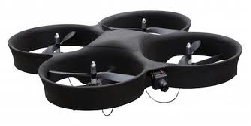
\includegraphics[width=0.3\textwidth]{figs/quadcopter.png}
\end{figure}
\item Automatic navigation using computer vision
\item Big map of Islamabad printed on panaflex
\item Navigation using down-looking camera
\end{itemize}
\begin{figure}
\centering
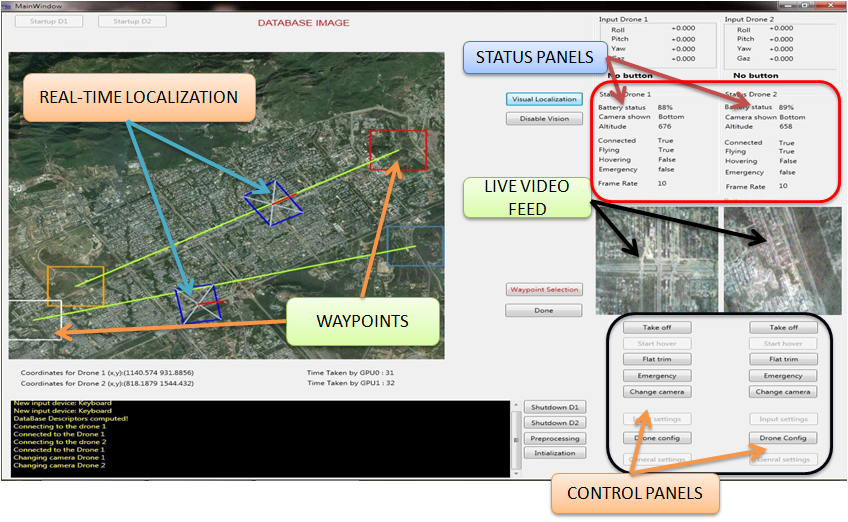
\includegraphics[width=0.8\textwidth]{figs/temp_Quadrotor_GUI.png}
\end{figure}
\end{frame}


\begin{frame}
\frametitle{CAE}
\framesubtitle{Robotics: 2. Mr Mansoor (2010)}
\mypagenum\ifthenelse{\boolean{ShowOverlays}}{\logoCAE}{}
\begin{itemize}
\item Autonomous flight using blimps
\begin{figure}
\centering
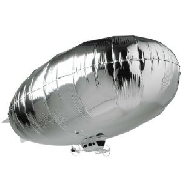
\includegraphics[width=0.3\textwidth]{figs/blimp.png}
\end{figure}
\end{itemize}
\end{frame}




\begin{frame}
\frametitle{CAE}
\framesubtitle{Robotics: 3.  Dr Salman Aslam (2012)}
\mypagenum\ifthenelse{\boolean{ShowOverlays}}{\logoCAE}{}
\begin{enumerate}\scriptsize
\item Autonomous helicopter
\begin{figure}
\centering
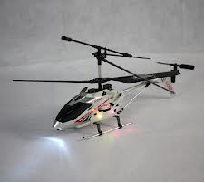
\includegraphics[width=0.3\textwidth]{figs/helicopter.png}
\end{figure}
\item Obstacle avoiding ground vehicle
\begin{figure}
\centering
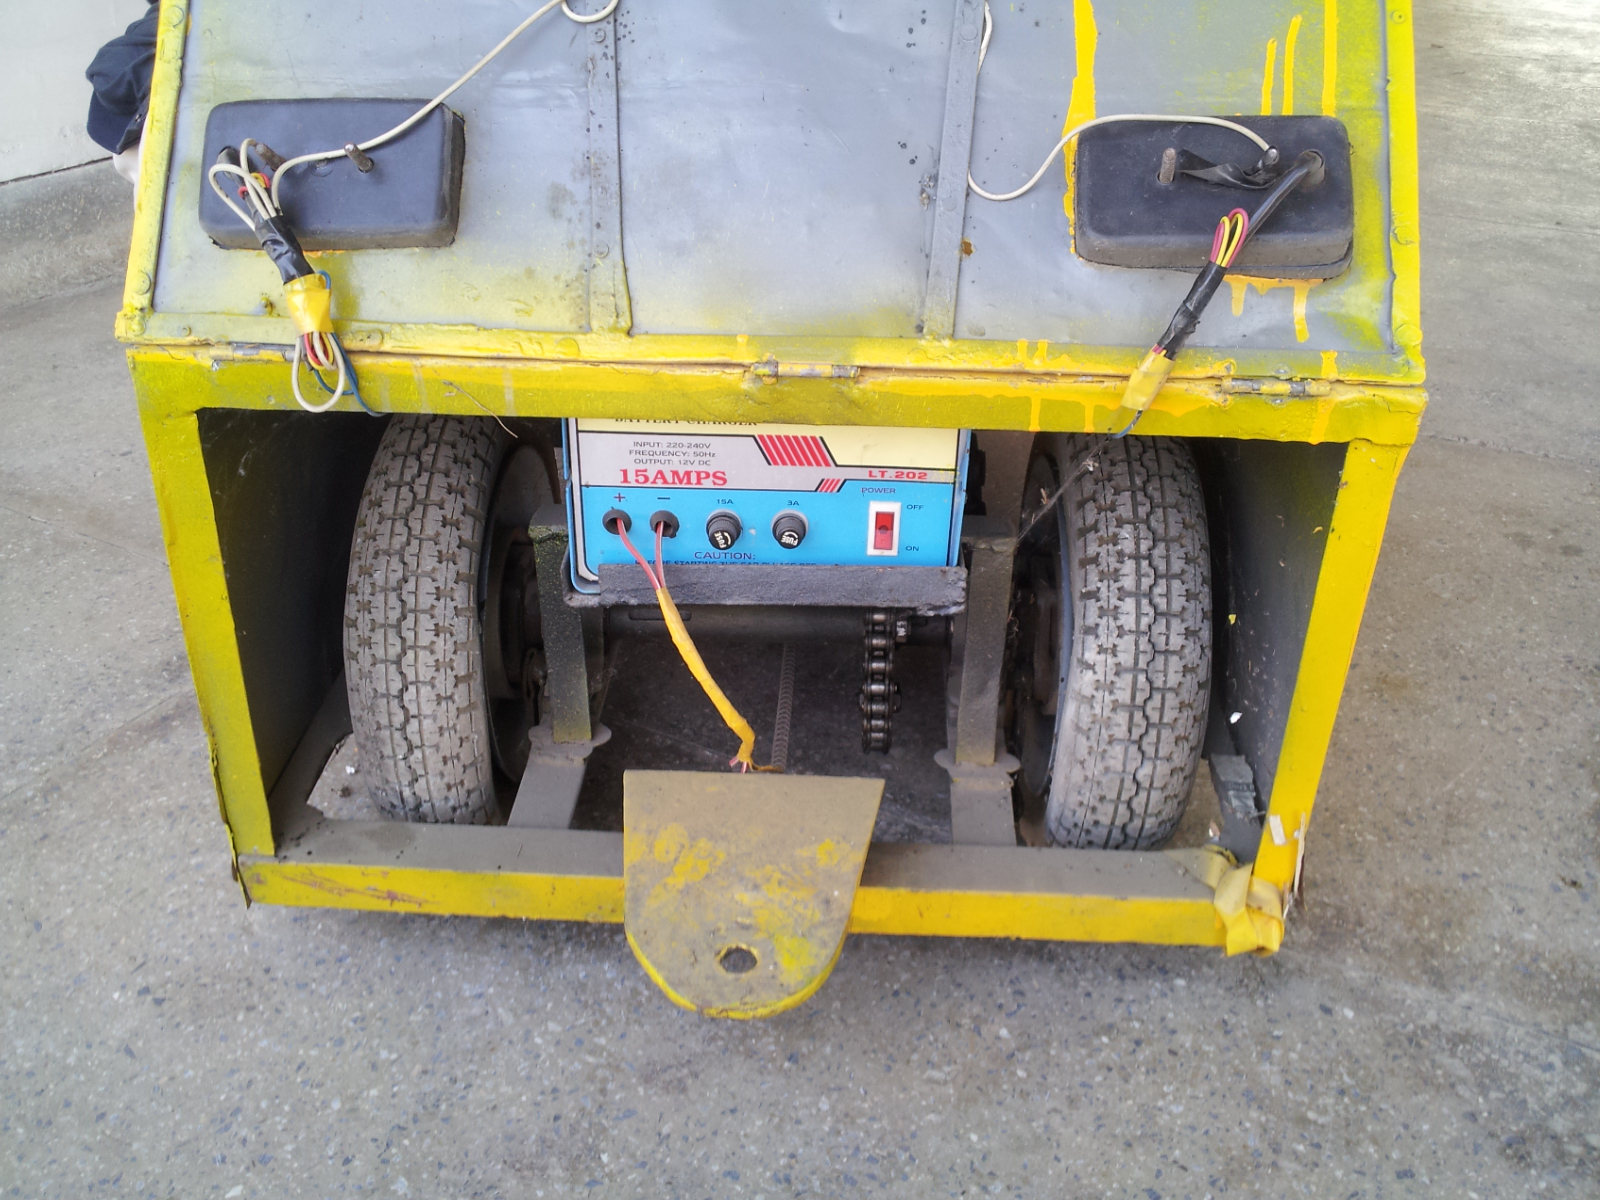
\includegraphics[width=0.3\textwidth]{figs/car.png}
\end{figure}
\item 3D surface reconstruction (for robotic applications, using Kinect)
\item 3D face recognition (security)
\item Controller design for CNC machine (manufacturing)
\end{enumerate}
\end{frame}







%####################################################################################################
\section{Target tracking using RVQ}
%####################################################################################################
%==========================
\subsection{\ \ \ \ Tracking}
%==========================

\begin{frame}
\frametitle{Tracking}
\framesubtitle{definition}
\mypagenum\ifthenelse{\boolean{ShowOverlays}}{\logoCAE}{}
Estimate and maintain {\color{red}target state} over {\color{red}time}
\begin{figure}
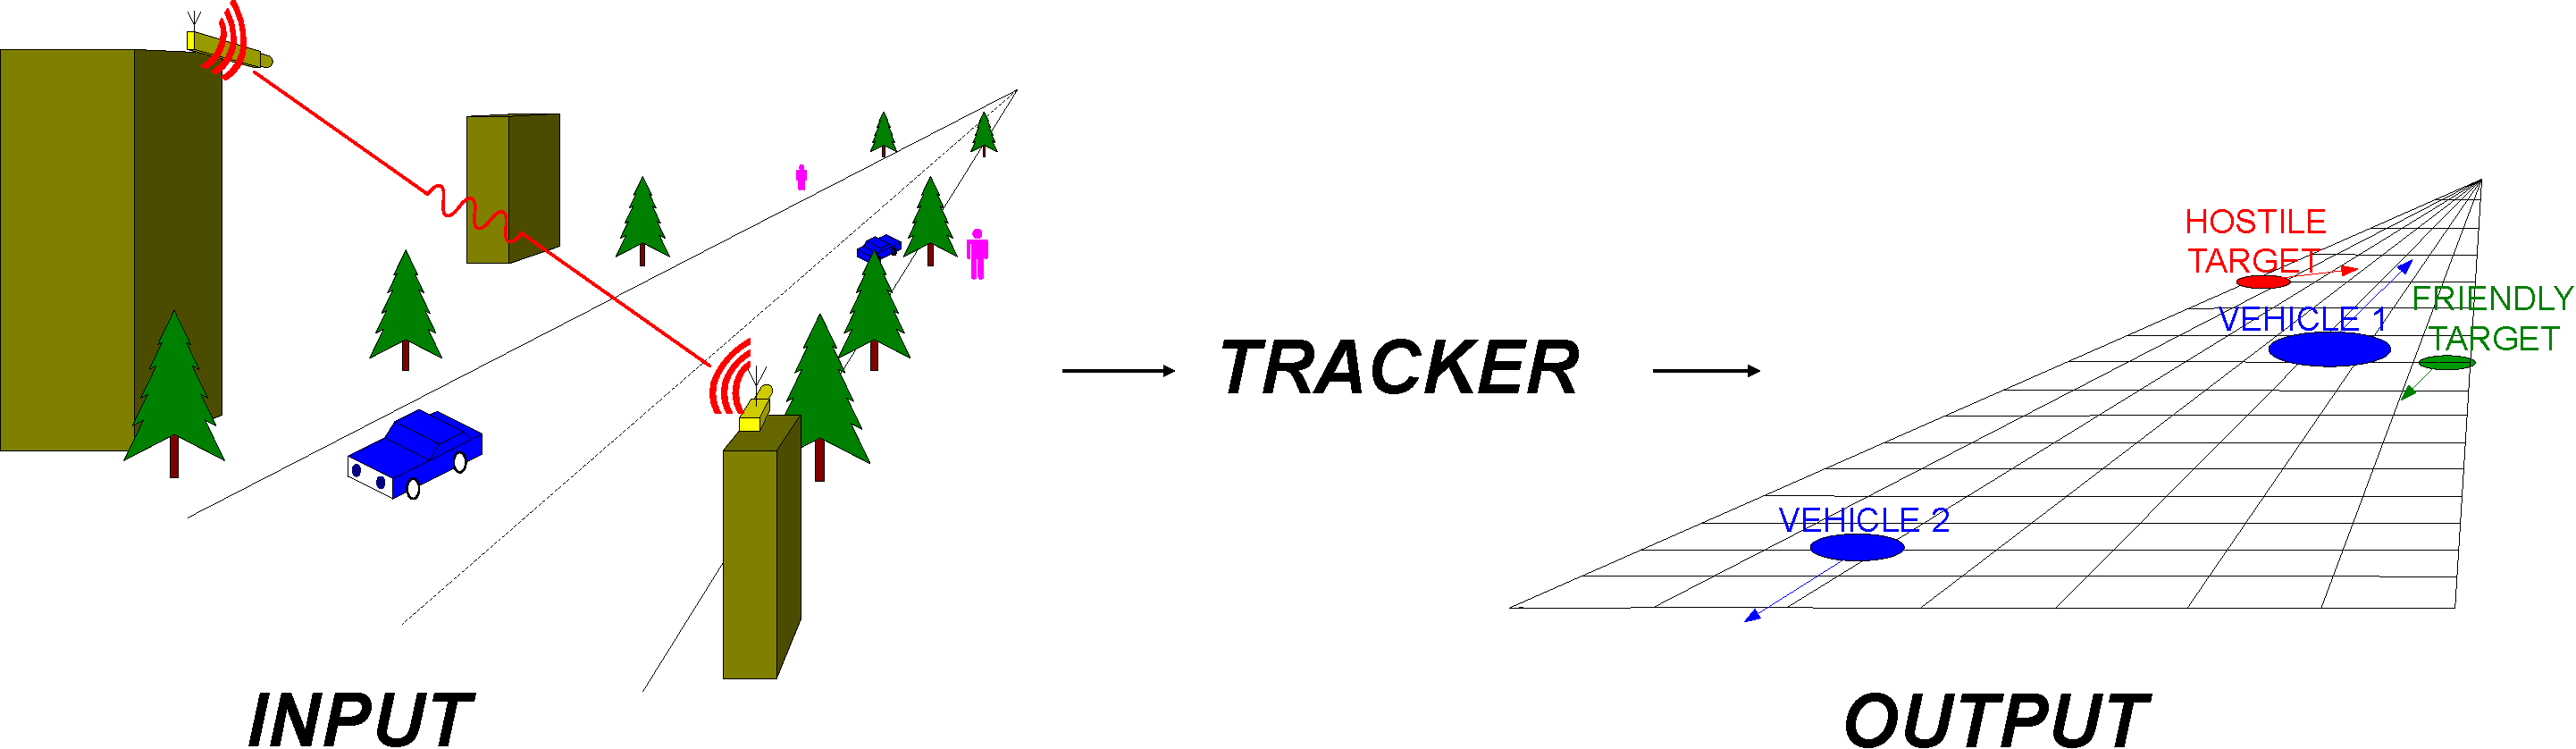
\includegraphics[width=1.0\textwidth]{figs/TRK_overviewDiagram.pdf}
\end{figure}
\vspace{0.2in}
2 step process
\begin{itemize}
\item Prediction: predict states using model
\item Update: correction applied to prediction after observation arrives
\end{itemize}
\end{frame}


\begin{frame}
\frametitle{Tracking}
\framesubtitle{Step 1 of 2: prediction (Chapman Kolmogorov)}
\mypagenum\ifthenelse{\boolean{ShowOverlays}}{\logoCAE}{}
\begin{table}
\begin{tabular}{|l|l|}\hline
$x_k$ & state at time $k$\\\hline
$Z_{k-1}$ &  all observations till time $k-1$\\\hline
\end{tabular}
\end{table}
\begin{figure}
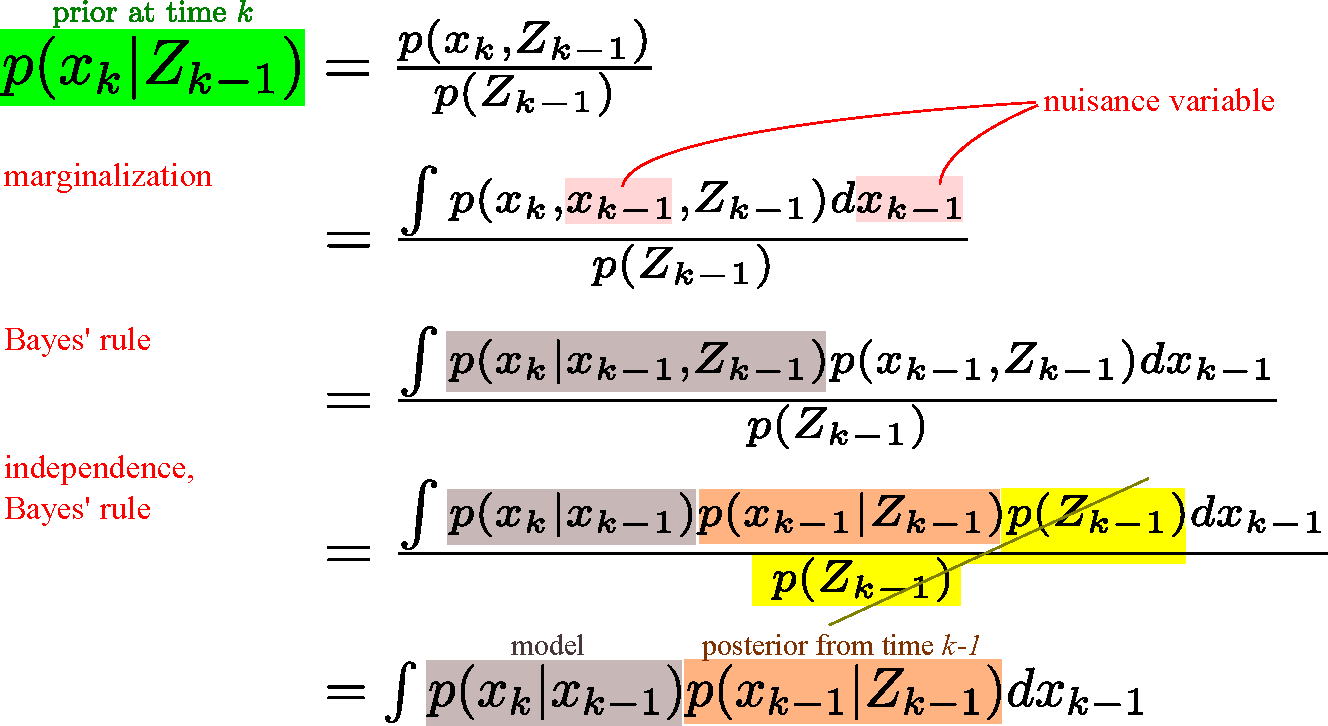
\includegraphics[width=1.0\textwidth]{figs/TRK_EQN_prediction.pdf}
\end{figure}
\end{frame}


\begin{frame}
\frametitle{Tracking}
\framesubtitle{Step 2 of 2: update}
\mypagenum\ifthenelse{\boolean{ShowOverlays}}{\logoCAE}{}
\begin{figure}
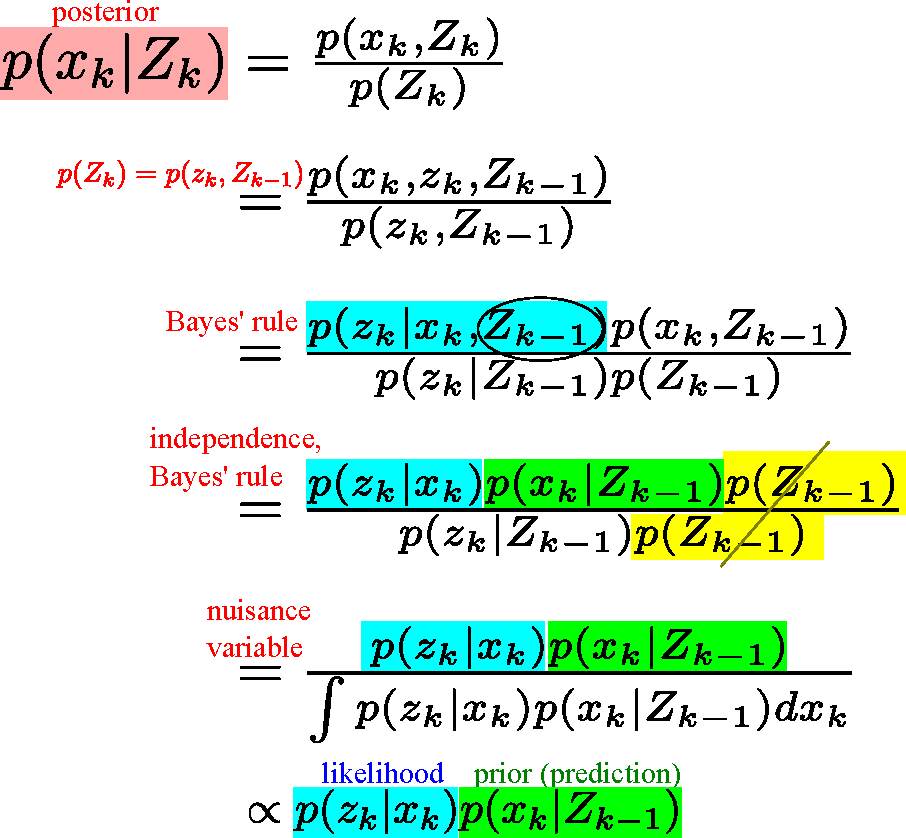
\includegraphics[height=0.8\textheight]{figs/TRK_EQN_update.pdf}
\end{figure}
\end{frame}


\begin{frame}
\frametitle{Tracking}
\framesubtitle{Example: 1D tracking with particle filter}
\mypagenum\ifthenelse{\boolean{ShowOverlays}}{\logoCAE}{}
\begin{figure}
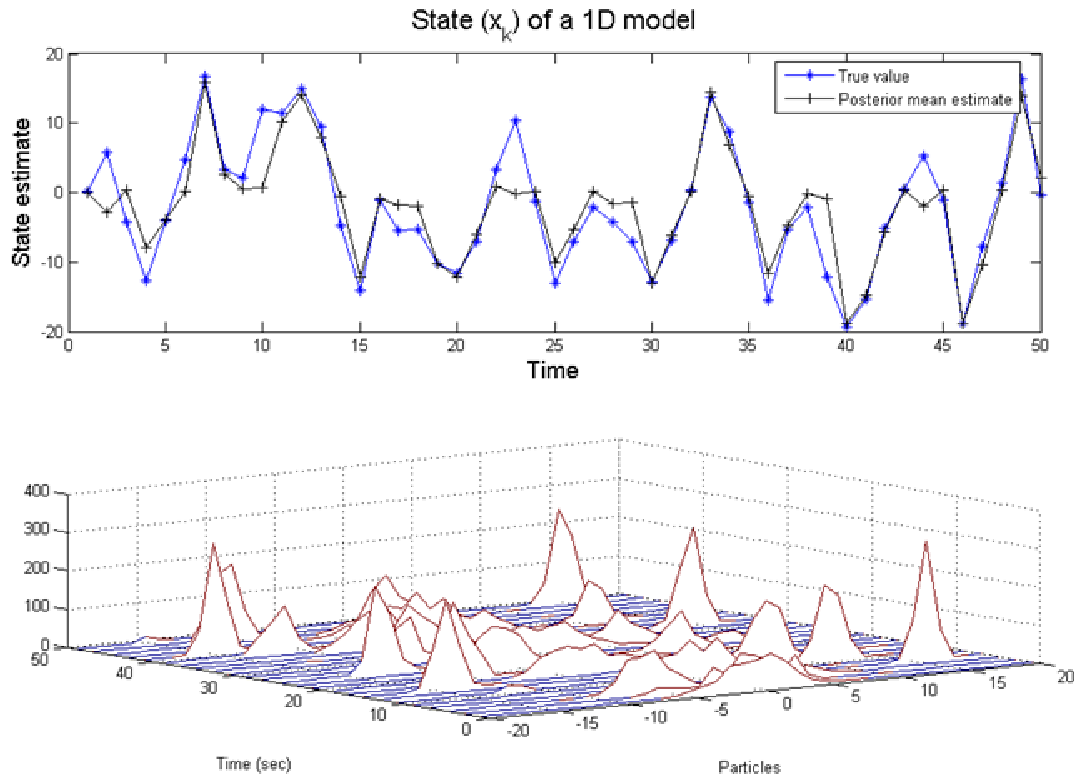
\includegraphics[width=1.0\textwidth]{figs/TRK_ParticleFilter_multimodalPDF.pdf}
\end{figure}	
\end{frame}



\begin{frame}
\frametitle{Tracking}
\framesubtitle{probabilistic graphical models}
\mypagenum\ifthenelse{\boolean{ShowOverlays}}{\logoCAE}{}
	\begin{figure}
		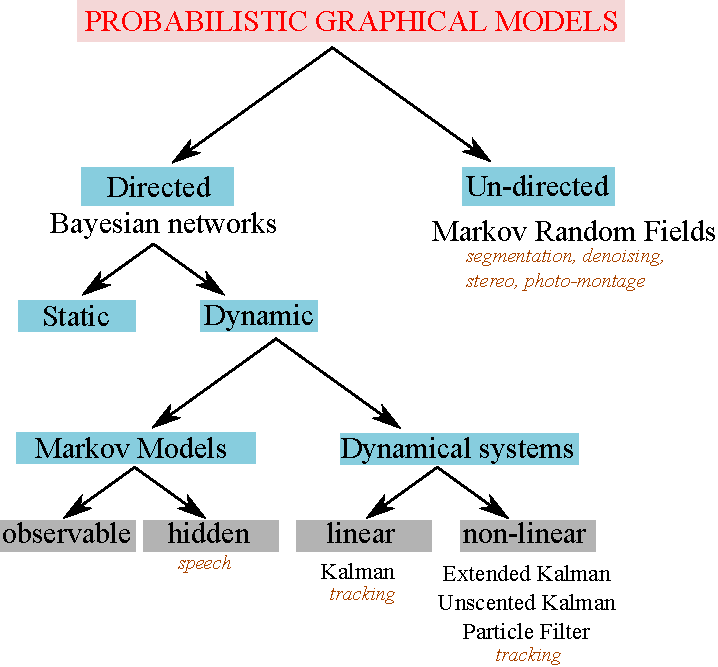
\includegraphics[width=0.9\textwidth]{figs/PRML_PGM_overview.pdf}
	\end{figure}
\end{frame}



\begin{frame}
\frametitle{Visual tracking}
\framesubtitle{components\tiny{\footnote {Yilmaz et.al., 2006}}}
\mypagenum\ifthenelse{\boolean{ShowOverlays}}{\logoCAE}{}
\begin{figure}
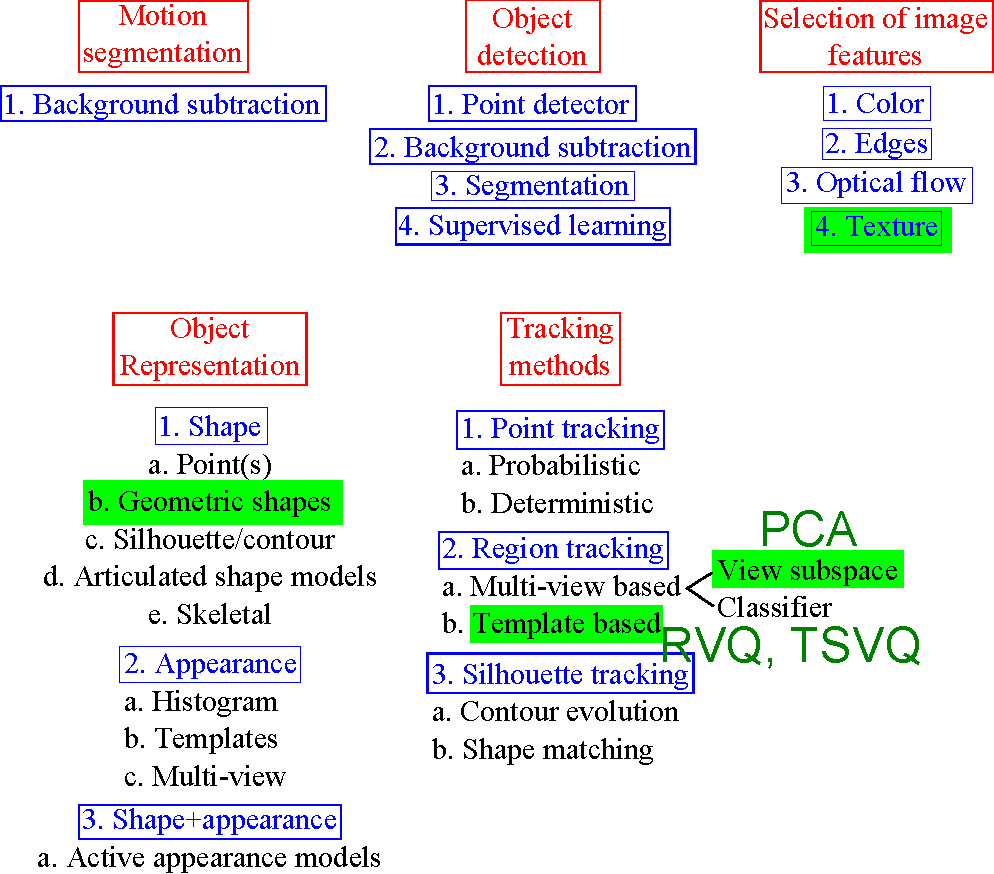
\includegraphics[height=0.8\textheight]{figs/TRK_overview.pdf}
\end{figure}	
\end{frame}


%==========================
\subsection{\ \ \ \ RVQ}
%==========================

\begin{frame}
\frametitle{RVQ}
\framesubtitle{}
\mypagenum\ifthenelse{\boolean{ShowOverlays}}{\logoCAE}{}
\vspace{0.2in}
\begin{itemize}\scriptsize
\item {\color{red}Vector Quantization}
\begin{itemize}\scriptsize
\item used in a variety of signal processing applications
\item design algorithm is known as Linde-Buzo-Gray (LBG) in signal processing community
\item known as K-means clustering in Computer Vision and PRML communities
\end{itemize}
\item {\color{red}Residual Vector Quantization}
\begin{itemize}\scriptsize
\item 1996: Developed by Dr Barnes (and later patented)
\item 2007: First successful application as a pattern recognition method for images
\end{itemize}
\end{itemize}
\begin{figure}
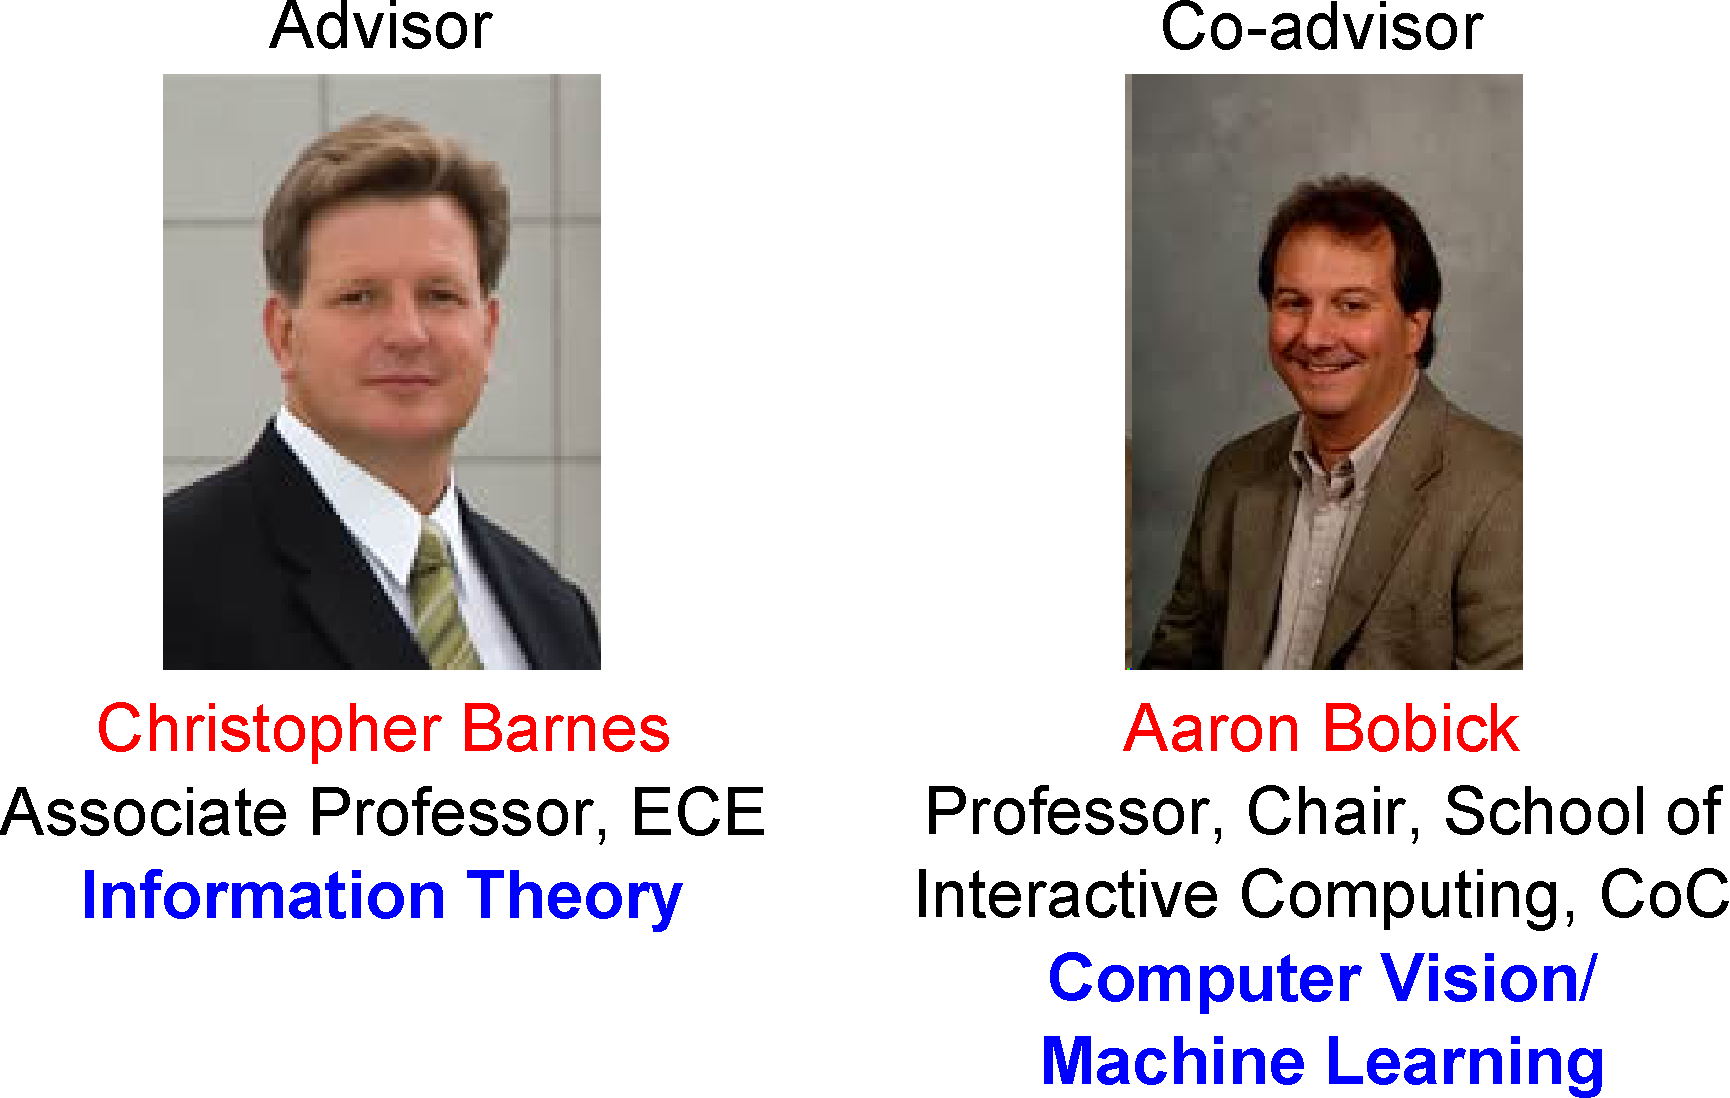
\includegraphics[width=0.73\textwidth]{figs/professors.pdf}
\end{figure}
\end{frame}


\begin{frame}
\frametitle{RVQ}
\framesubtitle{sample codebook (simple)}
\mypagenum\ifthenelse{\boolean{ShowOverlays}}{\logoCAE}{}
\begin{figure}[t]
\centering
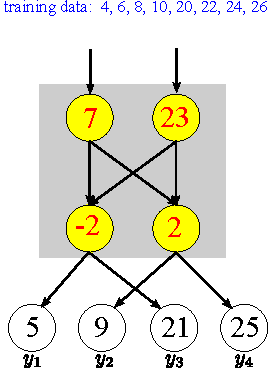
\includegraphics[width=0.5\textwidth]{figs/RVQ_introduction.pdf}
\end{figure}
\end{frame}


\begin{frame}
\frametitle{RVQ}
\framesubtitle{sample 8x4 codebook}
\logoCSIPCPL\mypagenum
\setcounter{subfigure}{0}
\begin{figure}[h!]
\centering\subfigure{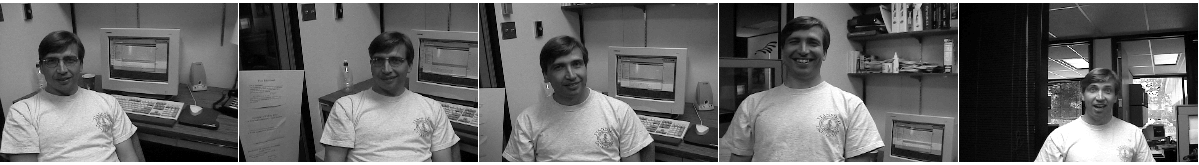
\includegraphics[height=0.41in]{figs/seq_1_Dudek.png}\label{fig:trk_pca_1a}}
\subfigure{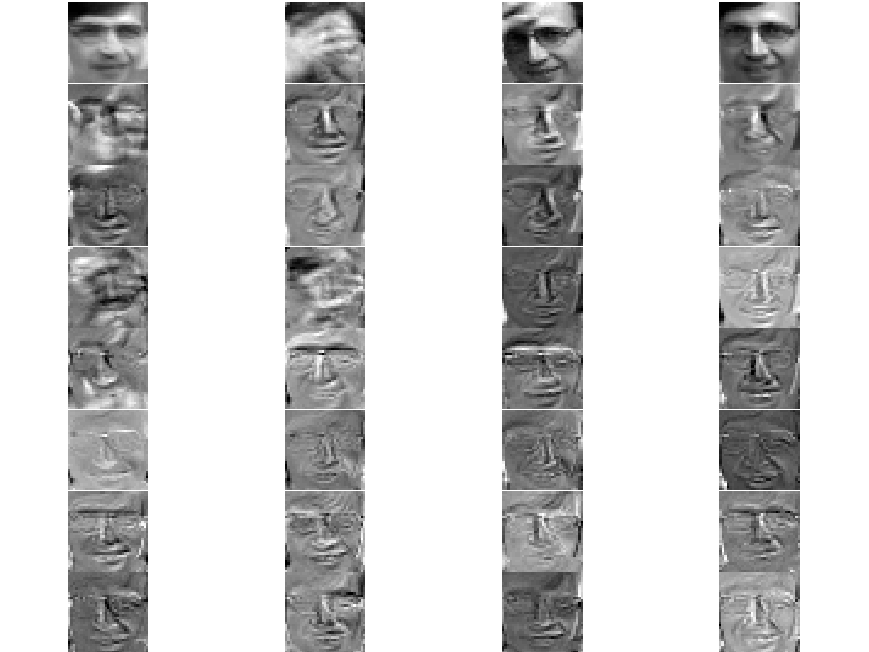
\includegraphics[height=0.65\textheight]{figs/1_Dudek__aRVQ_08_04_1000_0_RofE__170_codebook.pdf}
}
\end{figure}
\end{frame}



%==========================
\subsection{\ \ \ \ Prior work}
%==========================

\begin{frame}
\frametitle{Region tracking}
\framesubtitle{Subspace tracking: prior work}
\mypagenum\ifthenelse{\boolean{ShowOverlays}}{\logoCAE}{}
\vspace{0.1in}
1998: first work on subspace tracking
	\begin{figure}
		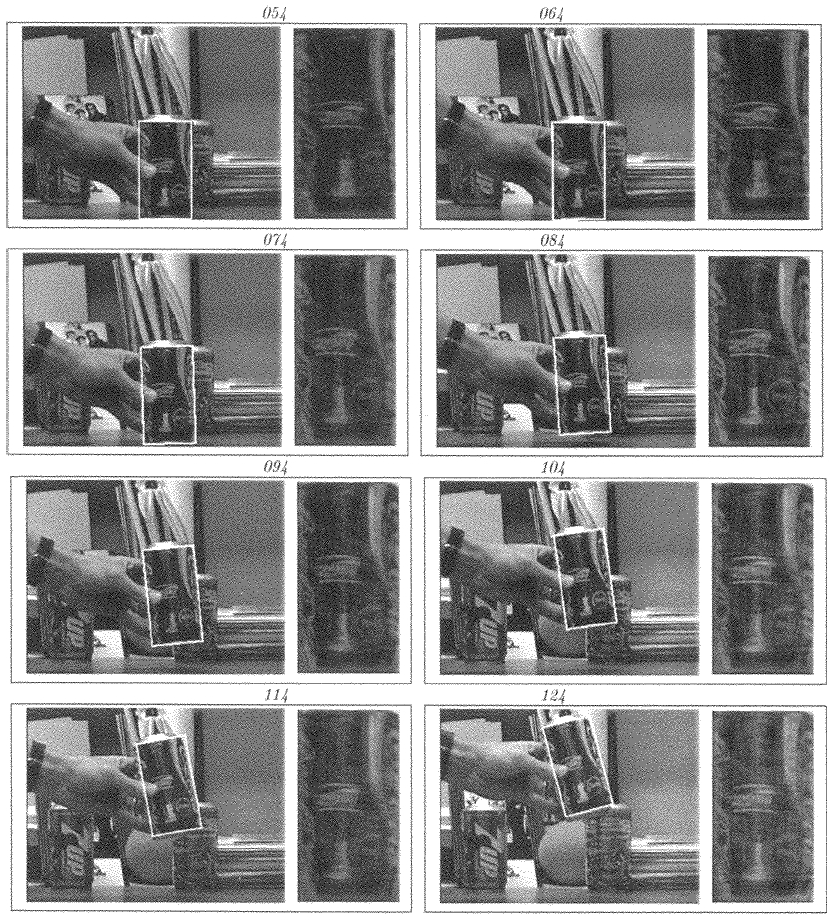
\includegraphics[width=0.6\textwidth]{figs/TrackingPapers_SubspaceTracking_1998_Black_fig9.png}
	\end{figure}
\myFootnoteCitation{1998_JNL_Eigentracking_Black}{IJCV}
\end{frame}


\begin{frame}
\frametitle{Region tracking}
\framesubtitle{Subspace tracking: prior work}
\logoCSIPCPL\mypagenum
\vspace{0.1in}
2008: 10 years later, state of the art in subspace tracking
\begin{figure}
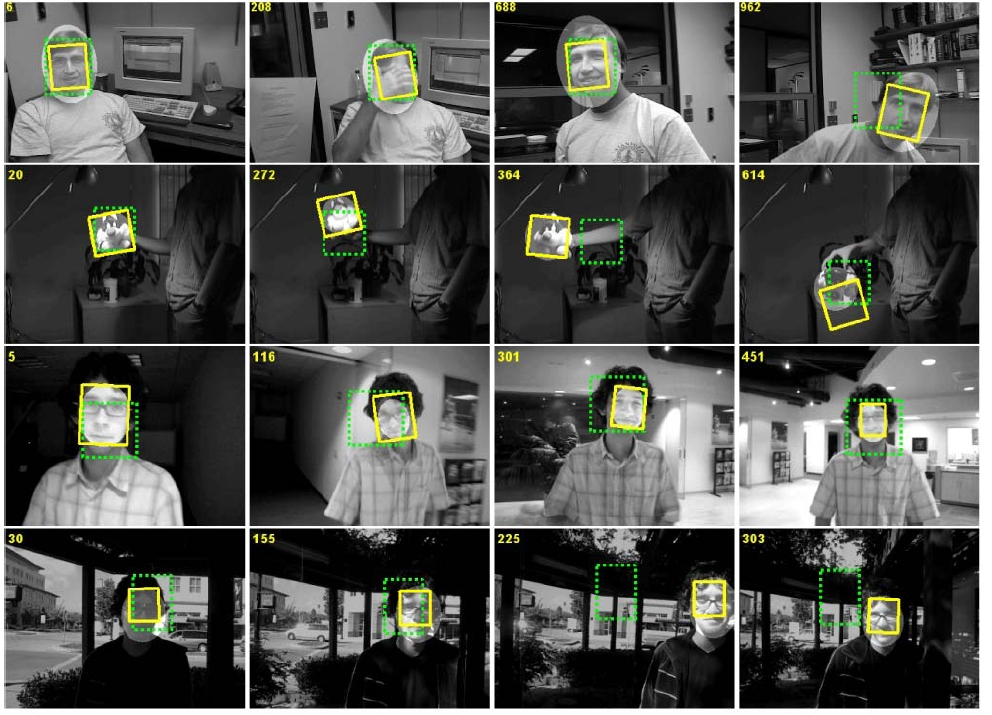
\includegraphics[width=0.9\textwidth]{figs/TrackingPapers_SubspaceTracking_2008_Ross_fig10.png}
\end{figure}
\myFootnoteCitation{2008_JNL_subspaceTRK_Ross}{IJCV}
\end{frame}





\begin{frame}
\frametitle{Image classification\footnote{Barnes, 2007}}
\framesubtitle{\small Satellite imagery: pre-Tsunami Sri Lanka \\(training phase)}
\mypagenum\ifthenelse{\boolean{ShowOverlays}}{\logoCAE}{}
	\begin{figure}		
		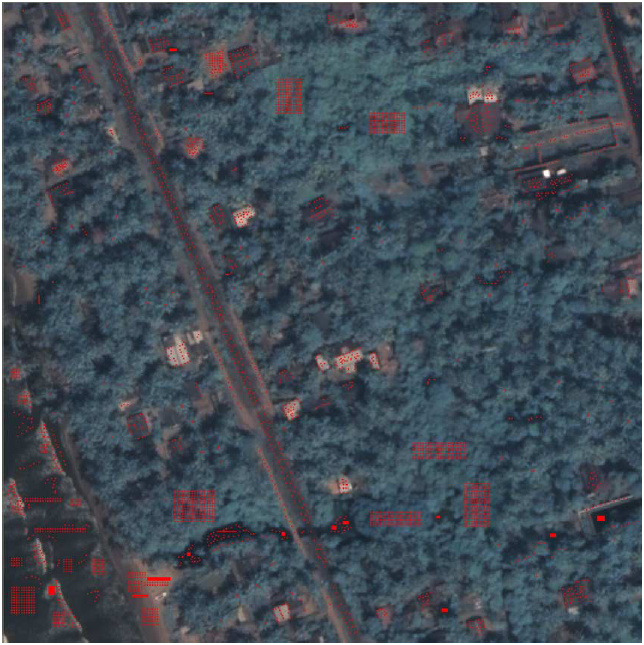
\includegraphics[height=0.3\textheight]{figs/RVQ_SatelliteSriLanka_1_snippets.png}			
	\end{figure}
	\begin{figure}		
		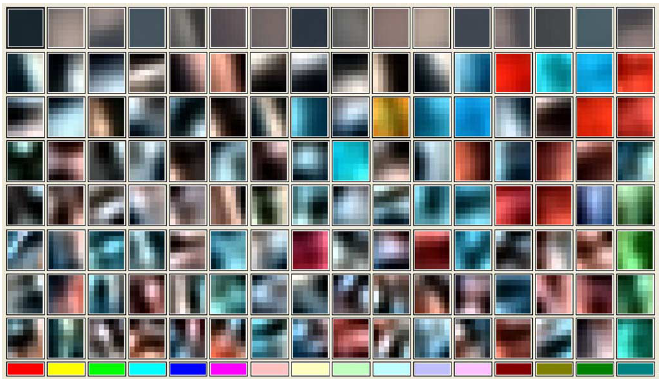
\includegraphics[height=0.35\textheight]{figs/RVQ_SatelliteSriLanka_2_codebooks.png}			
	\end{figure}
\end{frame}


%==========================
\subsection{\ \ \ \ Results}
%==========================

\begin{frame}
\frametitle{Publicly available datasets\footnote{Ross et. al. 2008}}
\framesubtitle{Dudek, davidin300, sylv, fish, car4, car11}
\mypagenum\ifthenelse{\boolean{ShowOverlays}}{\logoCAE}{}
\setcounter{subfigure}{0}
\begin{figure}[h!]
\centering\subfigure{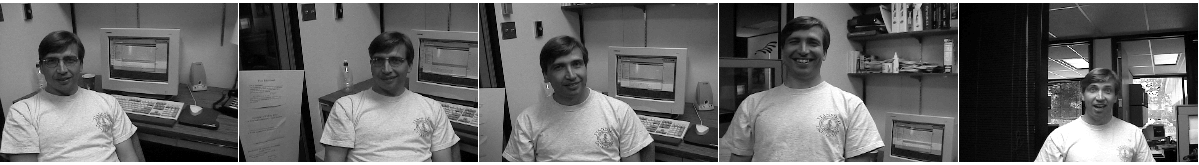
\includegraphics[height=0.41in]{figs/seq_1_Dudek.png}\label{fig:trk_pca_1a}}
\subfigure{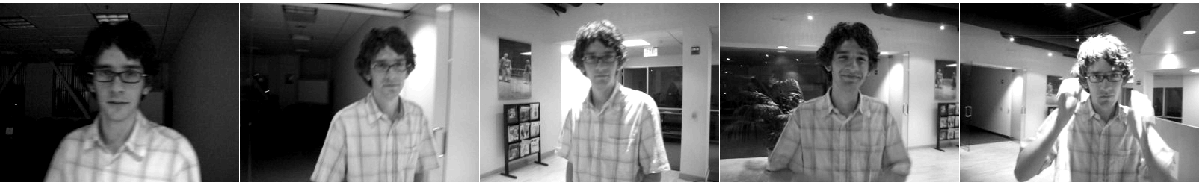
\includegraphics[height=0.41in]{figs/seq_2_davidin300.png}\label{fig:trk_pca_1b}}
\subfigure{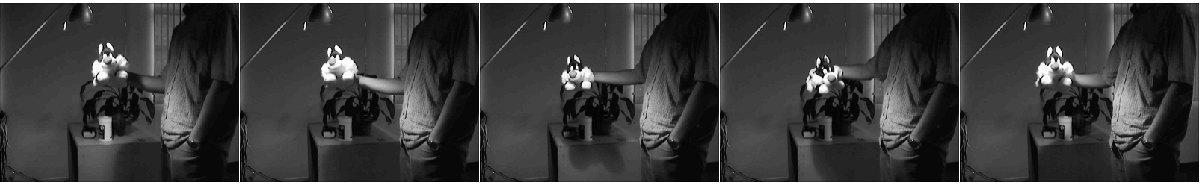
\includegraphics[height=0.41in]{figs/seq_3_sylv.png}\label{fig:trk_pca_1c}}
\subfigure{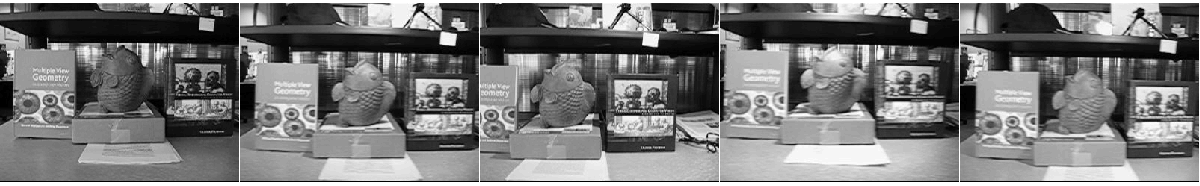
\includegraphics[height=0.41in]{figs/seq_5_fish.png}\label{fig:trk_pca_1d}}
\subfigure{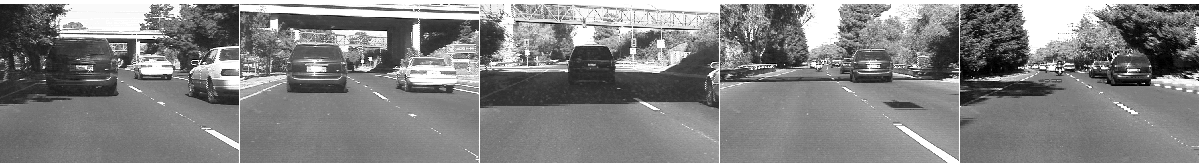
\includegraphics[height=0.41in]{figs/seq_6_car4.png}\label{fig:trk_pca_1d}}
\subfigure{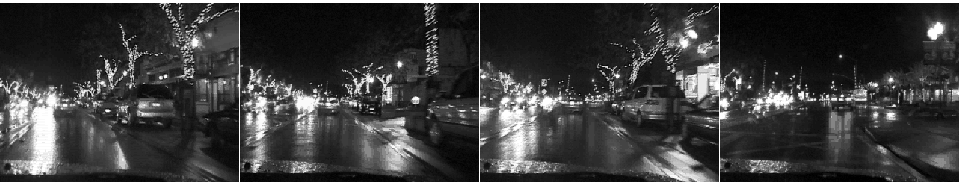
\includegraphics[height=0.41in]{figs/seq_7_car11.png}\label{fig:trk_pca_1d}}
\label{fig:trk_sequences}
\end{figure}
\end{frame}



\begin{frame}
\frametitle{Target motion}
\framesubtitle{Generating track candidates: run-time}
\mypagenum\ifthenelse{\boolean{ShowOverlays}}{\logoCAE}{}
Use random affine deformation to model motion
\begin{itemize}
\item Perturb affine parameters
\item For each affine set, 
\begin{itemize}
\item apply forward affine transform on zero-centered canonical grid 
\item bilinear interpolation to extract ROI, one per affine set, as shown below
\begin{figure}[t]
\centering
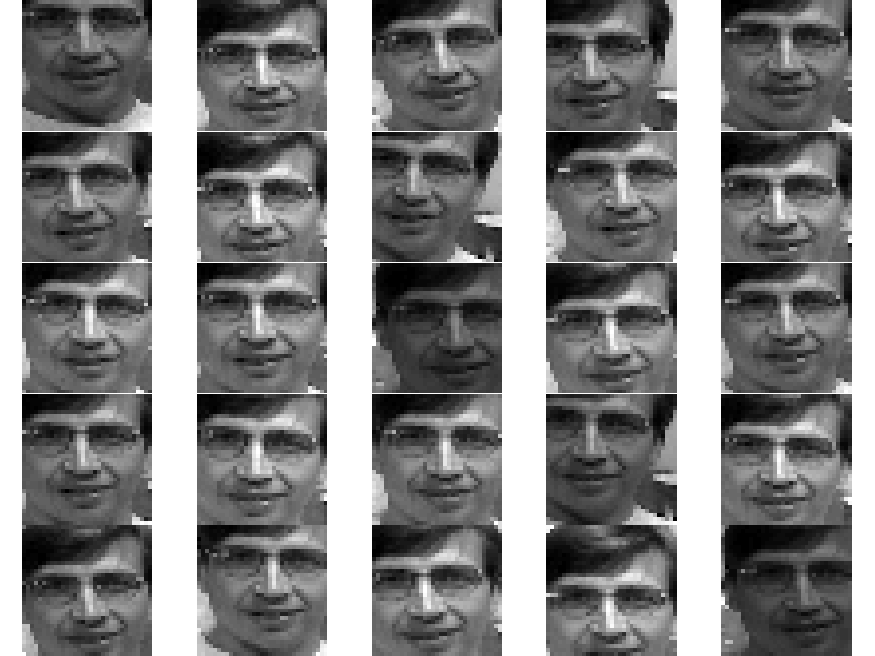
\includegraphics[width=0.35\textwidth]{figs/affineCandidates.pdf}
\label{Fig:affine_candidates}
\end{figure}
\end{itemize}
\item For set corresponding to least reconstruction error, apply forward affine transform to $(\mathbf{x, y})$ and compare with ground truth to get track error
\end{itemize}
\end{frame}



\begin{frame}
\frametitle{Results}
\framesubtitle{best tracking performance}
\mypagenum\ifthenelse{\boolean{ShowOverlays}}{\logoCAE}{}
\setcounter{subfigure}{0}
\begin{figure}[t]
\centering
\scriptsize
\begin{tabular}{|l|c|c|c|c|c|c|}
\hline
&\textbf{PCA}&\textbf{TSVQ}&\textbf{maxP}&\textbf{RofE}&\textbf{nulE}&\textbf{monR}\\\hline
\textbf{Dudek}&7.44&8.62&7.78&7.11&7.97&8.73\\\hline
\textbf{davidin300}&4.60&5.93&4.47&5.74&4.63&4.15\\\hline
\textbf{sylv}&4.34&4.61&4.00&4.12&4.74&4.31\\\hline
\textbf{fish}&2.17&4.59&2.78&2.73&2.48&2.89\\\hline
\textbf{car4}&4.60&5.11&4.67&4.93&5.28&4.71\\\hline
\textbf{car11}&2.13&2.21&2.17&2.33&2.52&2.47\\\hline
\textbf{ \% best}&50.00&0.00&16.67&16.67&0.00&16.67\\\hline
\end{tabular}

\subfigure[Best tracking error for each algorithm.]{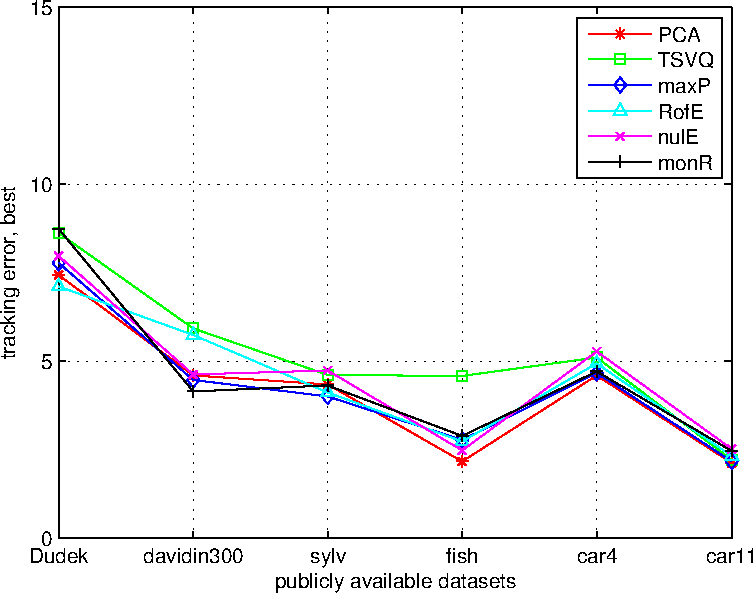
\includegraphics[width=0.47\textwidth]{figs/results_final_1a_best.pdf}\label{fig:results_final_1a_best}}\hspace{0.1in}
\subfigure[\%age of datasets over which best tracking error is achieved over all parameters.]{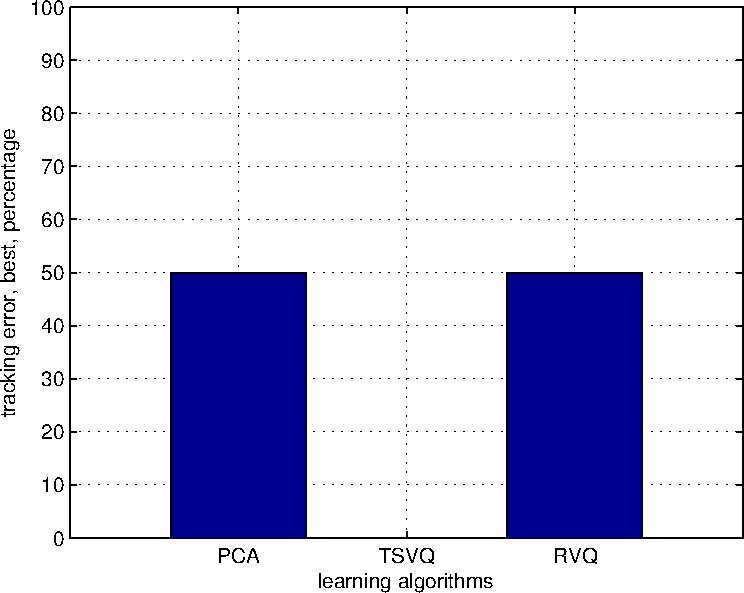
\includegraphics[width=0.47\textwidth]{figs/results_final_1b_best_percent.pdf}\label{fig:results_final_1b_best_percent}}
\end{figure}
\end{frame}



\begin{frame}
\frametitle{Results}
\framesubtitle{mean performance}
\mypagenum\ifthenelse{\boolean{ShowOverlays}}{\logoCAE}{}
\setcounter{subfigure}{0}
\begin{figure}[t]
\centering
\scriptsize
\begin{tabular}{|l|c|c|c|c|c|c|}
\hline
&\textbf{PCA}&\textbf{TSVQ}&\textbf{maxP}&\textbf{RofE}&\textbf{nulE}&\textbf{monR}\\\hline
\textbf{Dudek}&7.93&10.07&7.93&7.91&8.60&9.90\\\hline
\textbf{davidin300}&6.63&8.37&7.07&6.99&5.72&4.99\\\hline
\textbf{sylv}&5.18&4.70&4.47&4.83&5.10&4.66\\\hline
\textbf{fish}&6.63&6.71&8.81&5.97&5.74&6.15\\\hline
\textbf{car4}&4.97&5.90&5.38&5.19&5.77&4.99\\\hline
\textbf{car11}&2.24&3.48&2.70&2.49&2.69&2.58\\\hline
\textbf{ \% best}&33.33&0.00&16.67&16.67&16.67&16.67\\\hline
\end{tabular}

\subfigure[Mean tracking error for each algorithm.]{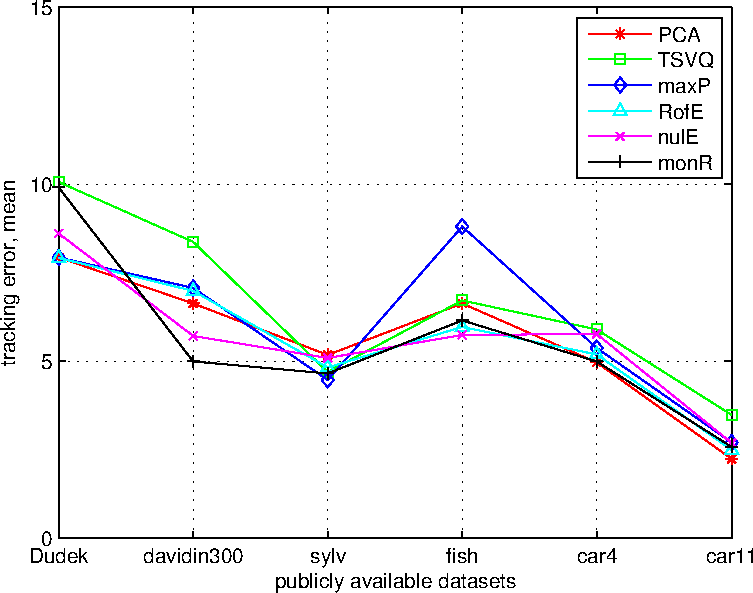
\includegraphics[width=0.47\textwidth]{figs/results_final_2a_mean.pdf}\label{fig:results_final_2a_mean}}\hspace{0.1in}
\subfigure[\%age of datasets over which best mean tracking error is achieved over all parameters.]{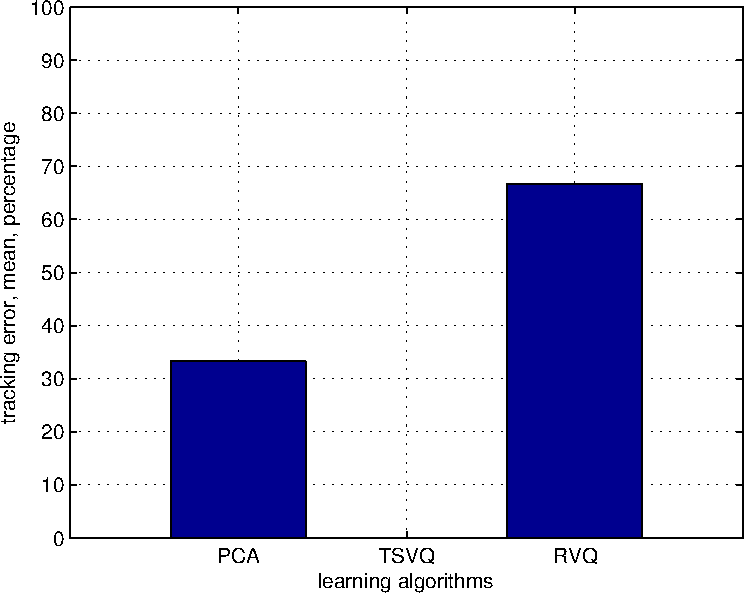
\includegraphics[width=0.47\textwidth]{figs/results_final_2b_mean_percent.pdf}\label{fig:results_final_2b_mean_percent}}
\label{fig:results_final_2_mean}
\end{figure}
\end{frame}


\begin{frame}
\frametitle{Results}
\framesubtitle{memory=16 vectors}
\mypagenum\ifthenelse{\boolean{ShowOverlays}}{\logoCAE}{}
\setcounter{subfigure}{0}
\begin{figure}[t]
\centering
\scriptsize
\begin{tabular}{|l|c|c|c|c|c|c|}
\hline
&\textbf{PCA}&\textbf{TSVQ}&\textbf{maxP}&\textbf{RofE}&\textbf{nulE}&\textbf{monR}\\\hline
\textbf{Dudek}&7.81&8.62&7.78&7.11&9.65&11.81\\\hline
\textbf{davidin300}&4.60&12.88&6.84&9.02&7.17&50.00\\\hline
\textbf{sylv}&5.47&4.70&4.00&4.12&4.81&4.31\\\hline
\textbf{fish}&2.17&10.07&11.50&2.96&4.03&2.89\\\hline
\textbf{car4}&4.60&5.11&4.67&4.93&5.28&5.07\\\hline
\textbf{car11}&2.13&2.21&2.17&2.47&2.59&2.47\\\hline
\textbf{ \% best}&66.67&0.00&16.67&16.67&0.00&0.00\\\hline
\end{tabular}

\subfigure[Tracking error for each algorithm with 16 eigenvectors/code-vectors stored in memory.]{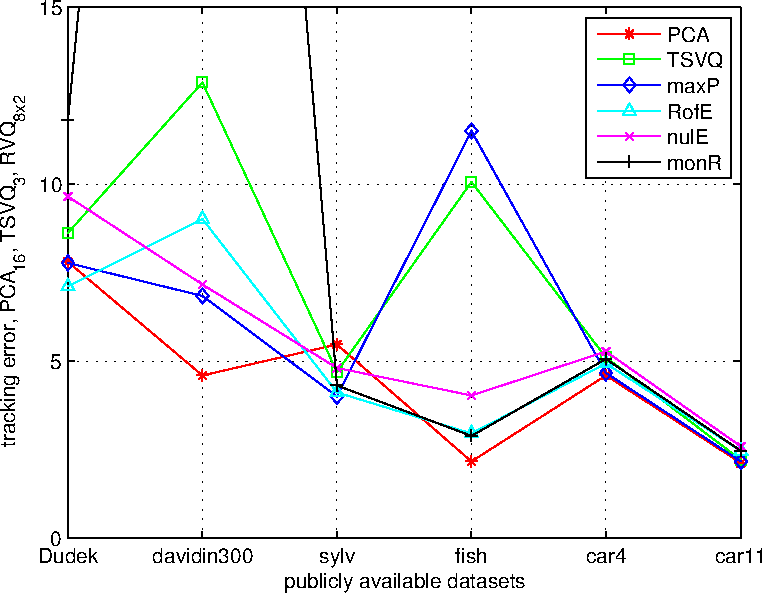
\includegraphics[width=0.47\textwidth]{figs/results_final_3a_16.pdf}\label{fig:results_final_3a_16}}\hspace{0.1in}
\subfigure[\%age of datasets over which best tracking error is achieved with 16 eigenvectors/code-vectors stored in memory.]{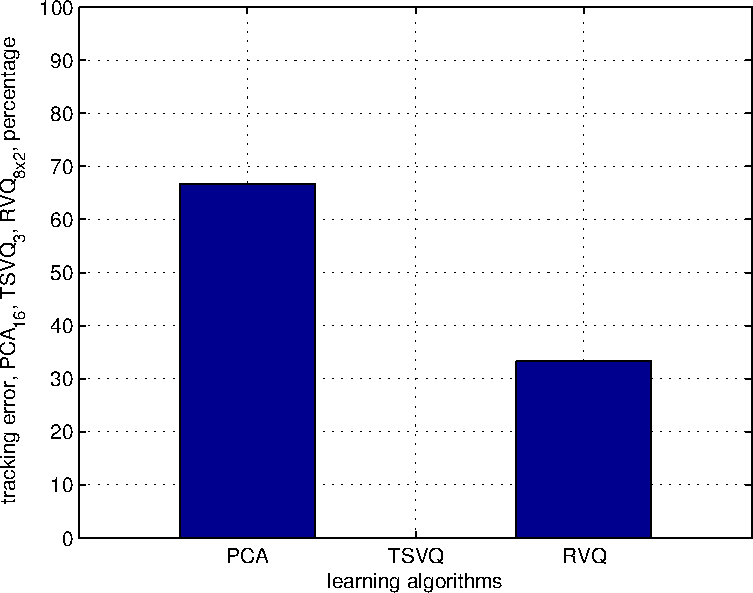
\includegraphics[width=0.47\textwidth]{figs/results_final_3b_16_percent.pdf}\label{fig:results_final_3b_16_percent}}
\label{fig:results_final_3_16}
\end{figure}
\end{frame}


\begin{frame}
\frametitle{Results}
\framesubtitle{memory=32 vectors}
\mypagenum\ifthenelse{\boolean{ShowOverlays}}{\logoCAE}{}
\setcounter{subfigure}{0}
\begin{figure}[t]
\centering
\scriptsize
\begin{tabular}{|l|c|c|c|c|c|c|}
\hline
&\textbf{PCA}&\textbf{TSVQ}&\textbf{maxP}&\textbf{RofE}&\textbf{nulE}&\textbf{monR}\\\hline
\textbf{Dudek}&8.54&11.87&7.92&8.43&8.19&9.17\\\hline
\textbf{davidin300}&6.93&6.29&4.47&6.21&5.35&5.83\\\hline
\textbf{sylv}&5.72&4.80&4.68&5.54&5.74&4.58\\\hline
\textbf{fish}&7.98&4.59&2.78&12.22&2.48&3.62\\\hline
\textbf{car4}&5.52&6.79&6.38&5.14&5.84&5.18\\\hline
\textbf{car11}&2.39&5.28&2.36&2.33&2.52&2.72\\\hline
\textbf{ \% best}&0.00&0.00&33.33&33.33&16.67&16.67\\\hline
\end{tabular}

\subfigure[Tracking error for each algorithm with 32 eigenvectors/code-vectors stored in memory.]{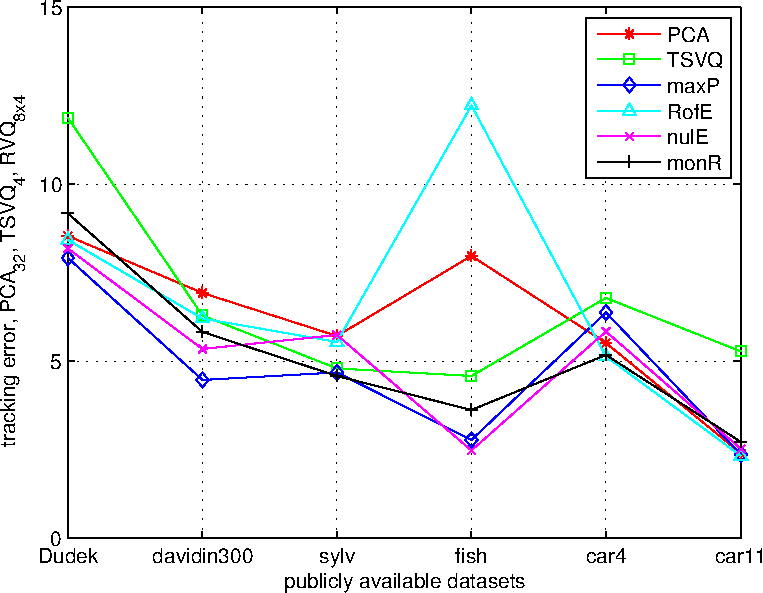
\includegraphics[width=0.47\textwidth]{figs/results_final_4a_32.pdf}\label{fig:results_final_4a_32}}\hspace{0.1in}
\subfigure[\%age of datasets over which best tracking error is achieved with 32 eigenvectors/code-vectors stored in memory.]{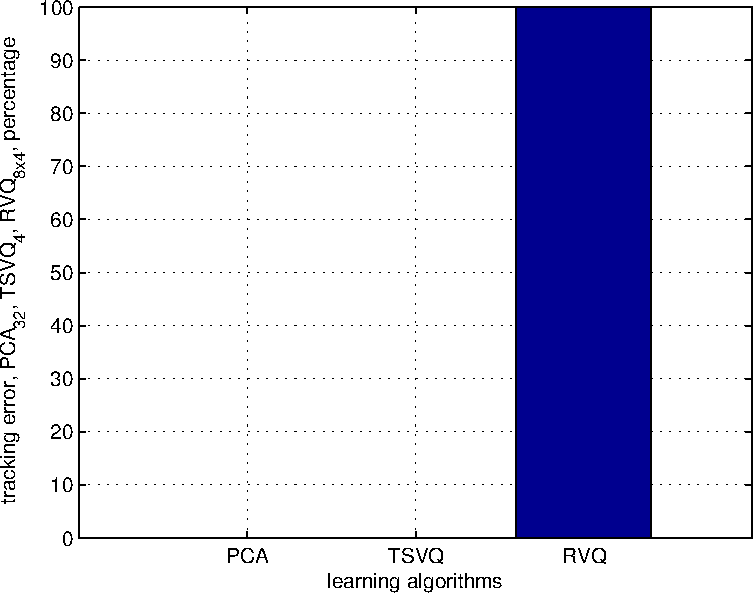
\includegraphics[width=0.47\textwidth]{figs/results_final_4b_32_percent.pdf}\label{fig:results_final_4b_32_percent}}
\label{fig:results_final_4_32}
\end{figure}
\end{frame}




\begin{frame}
\frametitle{Open source}
\framesubtitle{}
\mypagenum\ifthenelse{\boolean{ShowOverlays}}{\logoCAE}{}
\setcounter{subfigure}{0}
\begin{itemize}
\item All PhD work released under open source license
\item git clone, or download as zip
{\color{blue}\underline{\url{https://github.com/SalmanAslamPhD/phd}}}
\begin{figure}
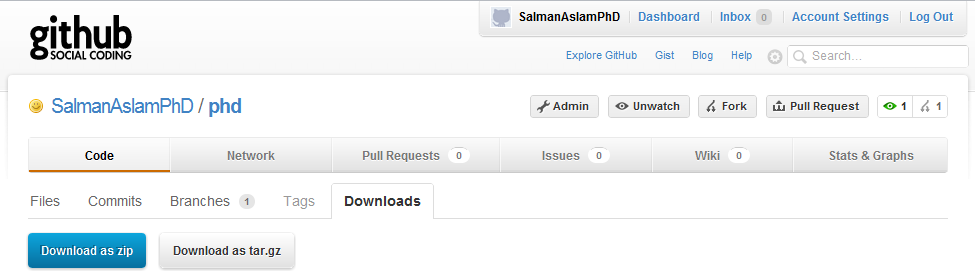
\includegraphics[width=0.9\textwidth]{figs/github.png}
\end{figure}
\item To run tracker, run main.m
\end{itemize}
\end{frame}





%####################################################################################################
\end{document}
%####################################################################################################

